\section{Data, per-benchmark results and figures}
\label{app:data}

\paragraph{Data and deduplication.}
All matrices come from the \texttt{data/scores} directory of the benchmark-prediction repository at commit \texttt{55faff496947789f94e6b5908c77cbc3e84f81ad} (MIT licence; see the checklist for upstream terms); only the 13 matrices, the seven \texttt{*\_models.jbl} lists and \texttt{helm\_model\_list.txt} are used. Table~\ref{tab:data} lists the models in the files; before splitting, exact duplicate model rows are collapsed (e.g.\ BBH 446$\to$425, MATH Lvl5 447$\to$375, ARC-C 218$\to$209; \texttt{results/sanity/data\_summary.csv}), which gives 20--107 target models per benchmark (25\%). Near-duplicate model pairs (response agreement $\ge99\%$) exist, mostly on MATH Lvl5 (2190 pairs) and GPQA (40), and may fall on either side of a split; we did not remove them. HELM score files ship no per-benchmark model list, so no family split was possible there.

\begin{table}[h]
\caption{Macro-average MAE (accuracy points) per benchmark at $n{=}50$ (\texttt{figures/generated/tab\_mae\_*\_n50.tex}). $\downarrow$/$\uparrow$: the paired difference to B1 has a 95\% interval below/above zero. Top: random split. Bottom: extrapolation split.}
\label{tab:perbench}
\centering
\resizebox{\linewidth}{!}{{\scriptsize\setlength{\tabcolsep}{2.5pt}
\begin{tabular}{lrrrrrrrrr}
\toprule
Benchmark & B1 random & B2 stratified & B3 rand.+cal. & Anchor points & Anchor+IRT & Random+low-rank & P1 OMP+ridge & P3 DR & P3 EB \\
\midrule
arc\_challenge & 5.86 & 3.77$^{\downarrow}$ & 3.37$^{\downarrow}$ & 8.99$^{\uparrow}$ & 2.73$^{\downarrow}$ & 2.91$^{\downarrow}$ & 2.27$^{\downarrow}$ & 3.49$^{\downarrow}$ & 3.11$^{\downarrow}$ \\
bbh & 5.44 & 4.56$^{\downarrow}$ & 4.36$^{\downarrow}$ & 4.05$^{\downarrow}$ & 3.32$^{\downarrow}$ & 3.13$^{\downarrow}$ & 2.01$^{\downarrow}$ & 3.95$^{\downarrow}$ & 3.22$^{\downarrow}$ \\
commonsense & 3.36 & 2.92$^{\downarrow}$ & 2.90$^{\downarrow}$ & 3.73 & 3.74$^{\uparrow}$ & 3.34 & 3.99$^{\uparrow}$ & 2.80$^{\downarrow}$ & 2.97$^{\downarrow}$ \\
gpqa & 5.06 & 4.72 & 2.64$^{\downarrow}$ & 5.52$^{\uparrow}$ & 2.40$^{\downarrow}$ & 1.91$^{\downarrow}$ & 1.29$^{\downarrow}$ & 4.11$^{\downarrow}$ & 2.87$^{\downarrow}$ \\
gsm & 4.07 & 3.52$^{\downarrow}$ & 3.54$^{\downarrow}$ & 4.47 & 4.33 & 3.85 & 6.22$^{\uparrow}$ & 3.51$^{\downarrow}$ & 3.51$^{\downarrow}$ \\
ifeval & 4.60 & 3.62$^{\downarrow}$ & 3.72$^{\downarrow}$ & 3.62$^{\downarrow}$ & 3.04$^{\downarrow}$ & 3.32$^{\downarrow}$ & 2.68$^{\downarrow}$ & 3.36$^{\downarrow}$ & 3.16$^{\downarrow}$ \\
legalbench & 5.26 & 4.37$^{\downarrow}$ & 4.13$^{\downarrow}$ & 3.09$^{\downarrow}$ & 3.80$^{\downarrow}$ & 3.76$^{\downarrow}$ & 4.17$^{\downarrow}$ & 3.58$^{\downarrow}$ & 3.28$^{\downarrow}$ \\
math & 4.40 & 3.64$^{\downarrow}$ & 3.68$^{\downarrow}$ & 3.79$^{\downarrow}$ & 4.31 & 4.19 & 6.10$^{\uparrow}$ & 3.67$^{\downarrow}$ & 3.64$^{\downarrow}$ \\
med\_qa & 5.11 & 4.02$^{\downarrow}$ & 4.04$^{\downarrow}$ & 3.75$^{\downarrow}$ & 3.78$^{\downarrow}$ & 3.78$^{\downarrow}$ & 5.81 & 3.81$^{\downarrow}$ & 3.58$^{\downarrow}$ \\
mmlu & 4.70 & 3.45$^{\downarrow}$ & 3.58$^{\downarrow}$ & 3.31$^{\downarrow}$ & 3.39$^{\downarrow}$ & 3.47$^{\downarrow}$ & 4.34 & 3.26$^{\downarrow}$ & 2.95$^{\downarrow}$ \\
mmlu\_pro & 4.53 & 3.81$^{\downarrow}$ & 3.46$^{\downarrow}$ & 3.92$^{\downarrow}$ & 3.04$^{\downarrow}$ & 2.76$^{\downarrow}$ & 1.81$^{\downarrow}$ & 3.45$^{\downarrow}$ & 2.97$^{\downarrow}$ \\
musr & 5.34 & 4.16$^{\downarrow}$ & 2.70$^{\downarrow}$ & 5.87 & 2.02$^{\downarrow}$ & 2.09$^{\downarrow}$ & 1.45$^{\downarrow}$ & 3.48$^{\downarrow}$ & 2.53$^{\downarrow}$ \\
openllm\_math & 2.10 & 1.79$^{\downarrow}$ & 1.68$^{\downarrow}$ & 1.82$^{\downarrow}$ & 1.19$^{\downarrow}$ & 1.81$^{\downarrow}$ & 1.22$^{\downarrow}$ & 1.71$^{\downarrow}$ & 1.72$^{\downarrow}$ \\
\midrule
macro & 4.60 & 3.72$^{\downarrow}$ & 3.37$^{\downarrow}$ & 4.30$^{\downarrow}$ & 3.16$^{\downarrow}$ & 3.10$^{\downarrow}$ & 3.33$^{\downarrow}$ & 3.40$^{\downarrow}$ & 3.04$^{\downarrow}$ \\
\bottomrule
\end{tabular}}
}\\[4pt]
\resizebox{\linewidth}{!}{{\scriptsize\setlength{\tabcolsep}{2.5pt}
\begin{tabular}{lrrrrrrrrr}
\toprule
Benchmark & B1 random & B2 stratified & B3 rand.+cal. & Anchor points & Anchor+IRT & Random+low-rank & P1 OMP+ridge & P3 DR & P3 EB \\
\midrule
arc\_challenge & 5.41 & 3.66$^{\downarrow}$ & 3.65$^{\downarrow}$ & 10.25$^{\uparrow}$ & 5.22 & 5.83 & 5.00 & 3.29$^{\downarrow}$ & 3.63$^{\downarrow}$ \\
bbh & 5.21 & 4.61$^{\downarrow}$ & 8.40$^{\uparrow}$ & 4.89 & 12.54$^{\uparrow}$ & 11.47$^{\uparrow}$ & 7.81$^{\uparrow}$ & 4.17$^{\downarrow}$ & 4.73$^{\downarrow}$ \\
commonsense & 2.42 & 1.92$^{\downarrow}$ & 2.52 & 1.87$^{\downarrow}$ & 4.90$^{\uparrow}$ & 5.84$^{\uparrow}$ & 3.15$^{\uparrow}$ & 1.88$^{\downarrow}$ & 2.30 \\
gpqa & 5.02 & 4.79 & 6.42$^{\uparrow}$ & 6.56$^{\uparrow}$ & 6.27$^{\uparrow}$ & 5.27$^{\uparrow}$ & 3.68$^{\downarrow}$ & 4.29$^{\downarrow}$ & 4.08$^{\downarrow}$ \\
gsm & 3.35 & 2.86$^{\downarrow}$ & 3.28 & 3.19 & 6.86$^{\uparrow}$ & 7.50$^{\uparrow}$ & 8.12$^{\uparrow}$ & 2.81$^{\downarrow}$ & 3.35 \\
ifeval & 4.73 & 4.24$^{\downarrow}$ & 6.88$^{\uparrow}$ & 7.58$^{\uparrow}$ & 9.57$^{\uparrow}$ & 13.05$^{\uparrow}$ & 8.43$^{\uparrow}$ & 4.04$^{\downarrow}$ & 4.63 \\
legalbench & 5.46 & 4.19$^{\downarrow}$ & 4.67 & 4.18$^{\downarrow}$ & 6.73$^{\uparrow}$ & 5.41 & 5.29 & 3.47$^{\downarrow}$ & 3.51$^{\downarrow}$ \\
math & 3.49 & 3.04$^{\downarrow}$ & 3.57 & 3.74 & 6.80$^{\uparrow}$ & 7.83$^{\uparrow}$ & 8.24$^{\uparrow}$ & 2.85$^{\downarrow}$ & 3.41 \\
med\_qa & 4.33 & 3.59$^{\downarrow}$ & 4.61 & 5.04$^{\uparrow}$ & 11.87$^{\uparrow}$ & 13.04$^{\uparrow}$ & 11.77$^{\uparrow}$ & 3.51$^{\downarrow}$ & 4.31 \\
mmlu & 4.49 & 3.51$^{\downarrow}$ & 4.03 & 5.10 & 7.71$^{\uparrow}$ & 8.25$^{\uparrow}$ & 5.92$^{\uparrow}$ & 3.25$^{\downarrow}$ & 3.78$^{\downarrow}$ \\
mmlu\_pro & 5.88 & 4.80$^{\downarrow}$ & 6.42 & 7.26$^{\uparrow}$ & 9.49$^{\uparrow}$ & 10.35$^{\uparrow}$ & 8.72$^{\uparrow}$ & 4.20$^{\downarrow}$ & 4.66$^{\downarrow}$ \\
musr & 5.24 & 4.24$^{\downarrow}$ & 5.45 & 6.50$^{\uparrow}$ & 4.75$^{\downarrow}$ & 4.32$^{\downarrow}$ & 2.33$^{\downarrow}$ & 3.55$^{\downarrow}$ & 3.33$^{\downarrow}$ \\
openllm\_math & 3.98 & 3.54$^{\downarrow}$ & 6.57$^{\uparrow}$ & 22.89$^{\uparrow}$ & 6.57$^{\uparrow}$ & 7.14$^{\uparrow}$ & 5.35$^{\uparrow}$ & 3.35$^{\downarrow}$ & 3.63 \\
\midrule
macro & 4.54 & 3.77$^{\downarrow}$ & 5.11$^{\uparrow}$ & 6.85$^{\uparrow}$ & 7.64$^{\uparrow}$ & 8.10$^{\uparrow}$ & 6.45$^{\uparrow}$ & 3.43$^{\downarrow}$ & 3.80$^{\downarrow}$ \\
\bottomrule
\end{tabular}}
}
\end{table}

\begin{figure}[h]
\centering
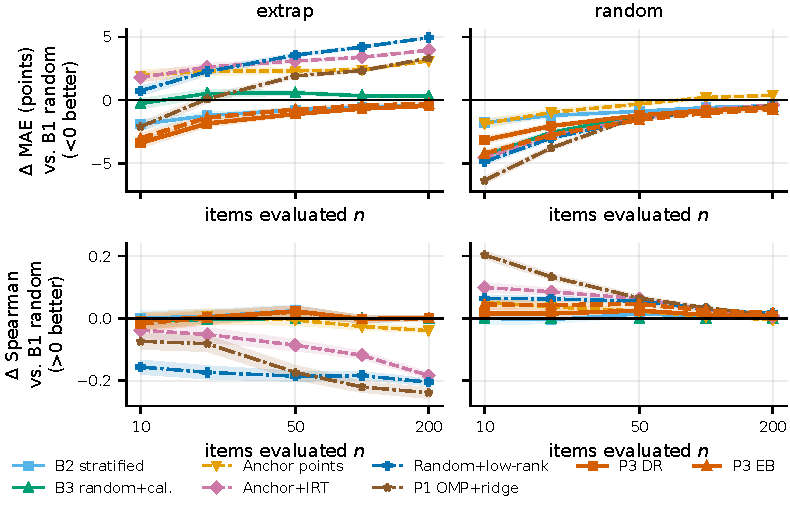
\includegraphics[width=\linewidth]{../figures/generated/fig_paired_diff.pdf}
\caption{Paired difference to the random subset mean (B1), macro-averaged over 13 benchmarks (95\% bootstrap bands). Top: MAE (negative is better); bottom: Spearman (positive is better). Left: extrapolation split; right: random split. $n{=}200$ covers 8 benchmarks.}
\label{fig:paired}
\end{figure}

\begin{figure}[h]
\centering
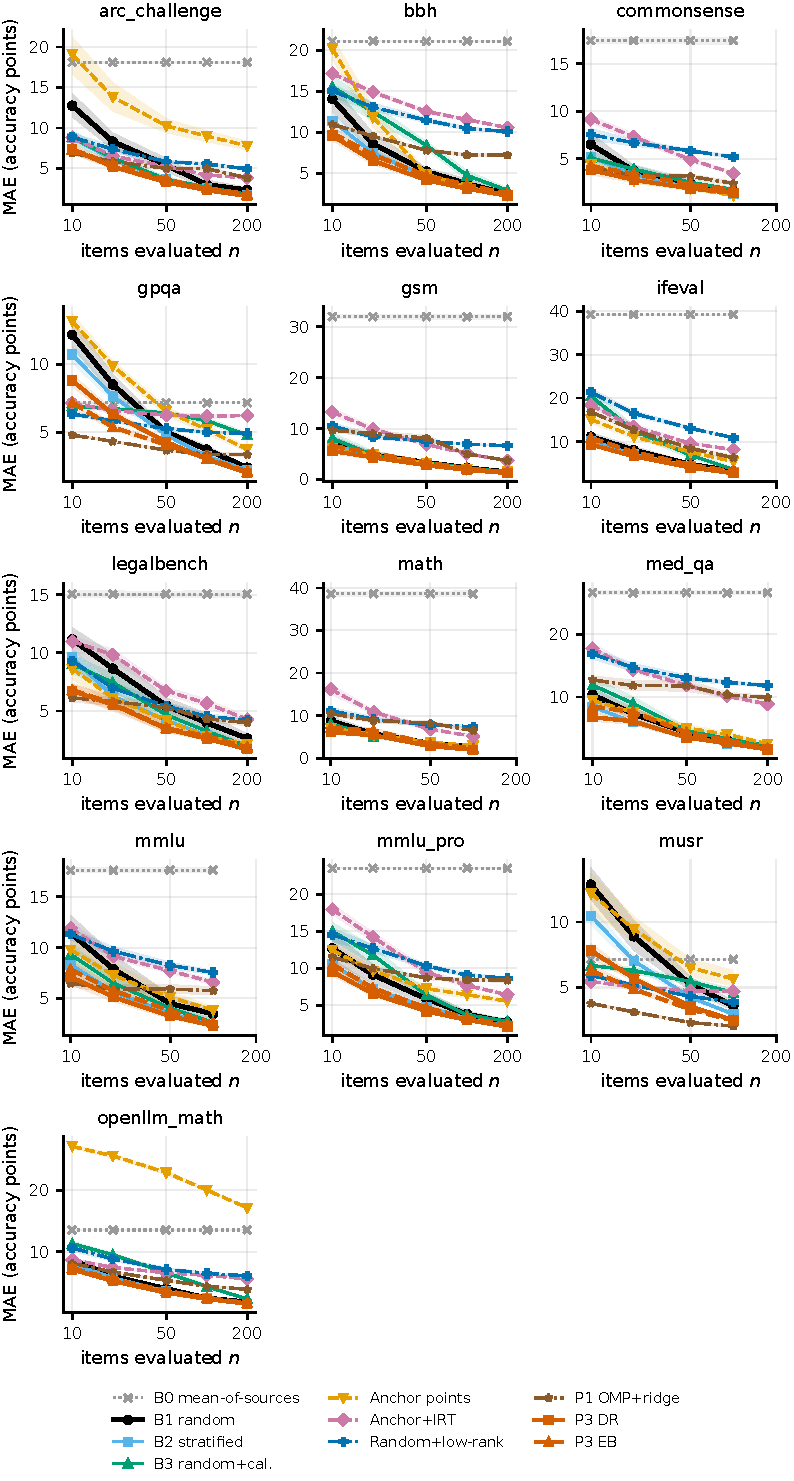
\includegraphics[width=0.8\linewidth]{../figures/generated/fig_mae_vs_n_extrap.pdf}
\caption{MAE against the number of items $n$, macro-average and per benchmark, extrapolation split, 95\% bands over repetitions. The same plot for the random split and the Spearman curves are in \texttt{figures/generated/}.}
\label{fig:curves}
\end{figure}

\begin{figure}[h]
\centering
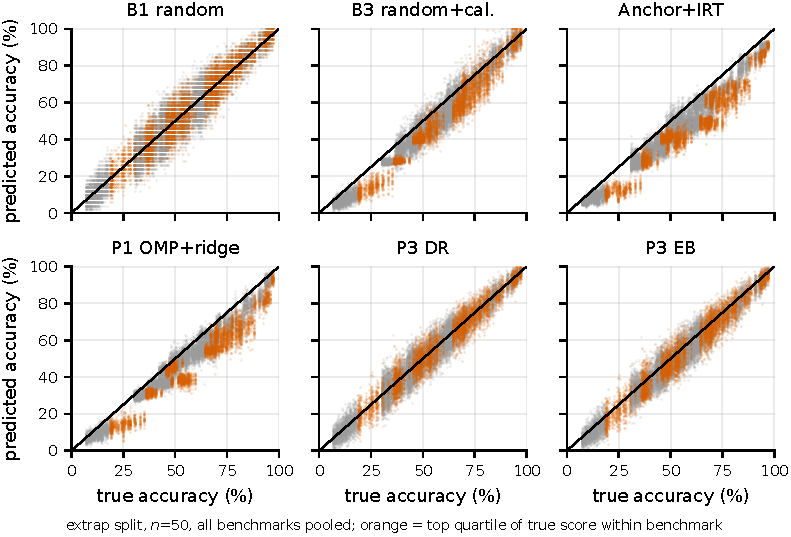
\includegraphics[width=0.8\linewidth]{../figures/generated/fig_scatter_extrap.pdf}
\caption{Predicted against true accuracy of target models, extrapolation split, $n{=}50$, all benchmarks pooled (orange: top quartile of true score within the benchmark).}
\label{fig:scatter}
\end{figure}

\begin{figure}[h]
\centering
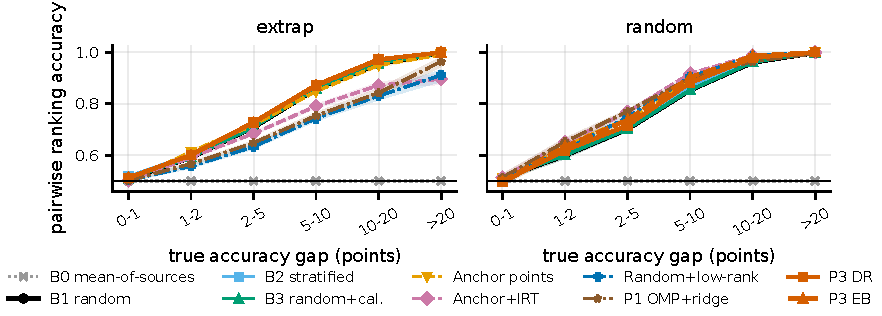
\includegraphics[width=0.9\linewidth]{../figures/generated/fig_pairwise_vs_gap.pdf}
\caption{Fraction of target-model pairs ordered correctly, by the true accuracy gap of the pair, $n{=}50$, macro-average over benchmarks.}
\label{fig:pairwise}
\end{figure}

\section{Further results}
\label{app:further}
\begin{table}[h]
\caption{Squared bias and variance of the prediction of a target model's accuracy over repetitions, in points$^2$, averaged over targets and benchmarks, $n{=}50$ (\texttt{paper/make\_tables.py} from \texttt{results/tables/tier1/q4\_bias\_variance.csv}). The squared bias of an unbiased design is not zero because it is estimated from a finite number of draws: $30$ on the extrapolation split, about $7.5$ on the random split (a model is a target in a quarter of the repetitions).}
\label{tab:q4}
\centering
{\scriptsize
\begin{tabular}{lrrrr}
\toprule
 & \multicolumn{2}{c}{random split} & \multicolumn{2}{c}{extrapolation} \\
\cmidrule(lr){2-3}\cmidrule(lr){4-5}
Method & bias$^2$ & variance & bias$^2$ & variance \\
\midrule
B0 mean of sources & 247.7 & 0.5 & 580.3 & 0.6 \\
B1 random & 5.1 & 29.9 & 1.2 & 32.2 \\
B2 stratified & 3.6 & 19.6 & 0.7 & 22.6 \\
B3 random + calibration & 5.6 & 13.5 & 25.7 & 13.4 \\
Anchor points & 13.7 & 18.9 & 109.3 & 23.2 \\
Anchor + IRT & 12.2 & 7.0 & 73.5 & 5.0 \\
Random + low-rank & 7.9 & 8.9 & 87.5 & 3.8 \\
P1 OMP + ridge & 9.2 & 18.3 & 57.6 & 7.3 \\
P3 DR (stratified + low-rank + correction) & 3.1 & 16.4 & 1.3 & 18.0 \\
P3 EB (shrunk correction) & 3.5 & 12.2 & 5.9 & 16.8 \\
\bottomrule
\end{tabular}}

\end{table}


\paragraph{Benchmark properties.}
Across the 13 benchmarks, the gain of P3 DR over B1 at $n{=}50$ (a negative MAE difference) is correlated with the spread of the item accuracies over source models (Spearman $-0.91$, bootstrap interval $[-0.99,-0.66]$ on the random split; $-0.82$, $[-0.95,-0.50]$ on the extrapolation split: more heterogeneous items, larger gain) and, positively, with the share of variance in the first singular component of the item matrix ($+0.62$ and $+0.65$; intervals exclude zero). The number of models, the number of items, the model-accuracy spread and the mean accuracy show no significant relation. This is descriptive: 13 benchmarks, nine properties examined per method without correction for multiplicity, and benchmarks that share models (\texttt{results/tables/tier1/q5\_benchmark\_properties.csv}).

\paragraph{Calibration of analytic intervals.}
As a by-product, we checked whether the nominal 95\% interval of a single model (finite-population standard error for B1, a Hajek residual standard error for the design-based estimators) covers the true score (Table~\ref{tab:coverage}). The pooled coverage is $0.86$ to $0.94$ and is below nominal at $n{=}20$ and on the random split (B1: $0.86$ at $n{=}20$ on the random split, $0.94$ at $n{=}100$ on the extrapolation split), so per-model analytic intervals are somewhat optimistic at small budgets. The intervals reported in this paper are bootstrap intervals over the study, not these.

\paragraph{All four metrics} (RMSE, Kendall and Spearman agree with MAE; Table~\ref{tab:metrics}).
\begin{table}[h]
\caption{Difference to B1 at $n{=}50$ in MAE, RMSE, Spearman and Kendall (macro-average over 13 benchmarks, 95\% two-level bootstrap intervals over repetitions and target models). Kendall's $\tau$ was bootstrapped over targets for seven methods only (dashes: not computed). Values from \texttt{results/tables/review/target\_bootstrap\_macro.csv}.}
\label{tab:metrics}\centering\resizebox{\linewidth}{!}{{\scriptsize\setlength{\tabcolsep}{3pt}
\begin{tabular}{lrrrr}
\toprule
Difference to B1 at $n{=}50$ & MAE (points) & RMSE (points) & Spearman & Kendall \\
\midrule
\multicolumn{5}{l}{\emph{random split}} \\
B2 stratified & -0.88\,{\tiny[-1.04,-0.73]} & -1.00\,{\tiny[-1.18,-0.83]} & +0.01\,{\tiny[+0.00,+0.03]} & +0.01\,{\tiny[+0.00,+0.03]} \\
B3 random + calibration & -1.23\,{\tiny[-1.36,-1.09]} & -1.44\,{\tiny[-1.56,-1.30]} & +0.00\,{\tiny[+0.00,+0.00]} & +0.00\,{\tiny[+0.00,+0.00]} \\
Anchor points & -0.30\,{\tiny[-0.50,-0.10]} & -0.35\,{\tiny[-0.57,-0.15]} & +0.02\,{\tiny[+0.01,+0.04]} & -- \\
Anchor + IRT & -1.44\,{\tiny[-1.60,-1.28]} & -1.54\,{\tiny[-1.75,-1.36]} & +0.06\,{\tiny[+0.05,+0.07]} & -- \\
Random + low-rank & -1.50\,{\tiny[-1.64,-1.35]} & -1.74\,{\tiny[-1.90,-1.57]} & +0.06\,{\tiny[+0.05,+0.06]} & +0.04\,{\tiny[+0.03,+0.05]} \\
P1 OMP + ridge & -1.27\,{\tiny[-1.45,-1.09]} & -1.17\,{\tiny[-1.45,-0.98]} & +0.07\,{\tiny[+0.05,+0.08]} & -- \\
Random + low-rank + correction & -1.13\,{\tiny[-1.26,-0.99]} & -1.28\,{\tiny[-1.42,-1.13]} & +0.02\,{\tiny[+0.01,+0.02]} & +0.00\,{\tiny[-0.00,+0.01]} \\
P3 DR & -1.20\,{\tiny[-1.36,-1.05]} & -1.37\,{\tiny[-1.54,-1.20]} & +0.02\,{\tiny[+0.01,+0.04]} & +0.01\,{\tiny[+0.00,+0.02]} \\
P3 EB & -1.56\,{\tiny[-1.72,-1.40]} & -1.81\,{\tiny[-1.97,-1.63]} & +0.05\,{\tiny[+0.04,+0.06]} & +0.04\,{\tiny[+0.02,+0.05]} \\
\multicolumn{5}{l}{\emph{extrapolation split}} \\
B2 stratified & -0.77\,{\tiny[-0.95,-0.61]} & -0.83\,{\tiny[-1.01,-0.65]} & +0.02\,{\tiny[+0.00,+0.05]} & +0.02\,{\tiny[+0.00,+0.04]} \\
B3 random + calibration & +0.58\,{\tiny[+0.38,+0.77]} & +0.39\,{\tiny[+0.20,+0.59]} & +0.00\,{\tiny[-0.00,+0.00]} & +0.00\,{\tiny[-0.00,+0.00]} \\
Anchor points & +2.31\,{\tiny[+2.11,+2.52]} & +3.07\,{\tiny[+2.85,+3.26]} & -0.00\,{\tiny[-0.03,+0.01]} & -- \\
Anchor + IRT & +3.10\,{\tiny[+2.91,+3.28]} & +2.94\,{\tiny[+2.75,+3.13]} & -0.09\,{\tiny[-0.11,-0.06]} & -- \\
Random + low-rank & +3.56\,{\tiny[+3.37,+3.74]} & +3.50\,{\tiny[+3.32,+3.69]} & -0.19\,{\tiny[-0.21,-0.16]} & -0.17\,{\tiny[-0.19,-0.15]} \\
P1 OMP + ridge & +1.91\,{\tiny[+1.71,+2.12]} & +1.98\,{\tiny[+1.77,+2.21]} & -0.17\,{\tiny[-0.20,-0.14]} & -- \\
Random + low-rank + correction & -0.99\,{\tiny[-1.14,-0.83]} & -1.07\,{\tiny[-1.24,-0.92]} & -0.00\,{\tiny[-0.01,+0.00]} & -0.02\,{\tiny[-0.03,-0.01]} \\
P3 DR & -1.10\,{\tiny[-1.27,-0.94]} & -1.21\,{\tiny[-1.39,-1.05]} & +0.02\,{\tiny[-0.00,+0.04]} & +0.00\,{\tiny[-0.02,+0.02]} \\
P3 EB & -0.74\,{\tiny[-0.92,-0.58]} & -0.85\,{\tiny[-1.03,-0.66]} & +0.02\,{\tiny[-0.00,+0.04]} & -0.00\,{\tiny[-0.02,+0.02]} \\
\bottomrule
\end{tabular}}
}
\end{table}

\paragraph{Tables of the further analyses} (organisation hold-out, selector$\times$estimator, number of source models, rank of the latent model, interval coverage; Section~\ref{sec:exp}).
\begin{table}[h]
\caption{Macro MAE (points) at $n{=}50$ on the four Open LLM Leaderboard benchmarks, 20 repetitions, for three kinds of split.}
\label{tab:family}\centering{\scriptsize
\begin{tabular}{lrrr}
\toprule
Method & random & organisation hold-out & extrapolation \\
\midrule
B1 random & 4.91 & 4.87 & 5.21 \\
B2 stratified & 4.18 & 4.20 & 4.61 \\
B3 random+calib. & 3.55 & 3.55 & 7.03 \\
Anchor points & 4.27 & 4.43 & 6.58 \\
Anchor+IRT & 2.95 & 3.06 & 9.47 \\
Random+low-rank & 2.78 & 2.88 & 10.04 \\
OMP+ridge & 1.95 & 2.20 & 7.16 \\
Random+low-rank+corr. & 3.76 & 3.76 & 4.30 \\
P3 DR & 3.72 & 3.73 & 4.18 \\
P3 EB & 3.06 & 3.09 & 4.52 \\
\bottomrule
\end{tabular}}

\end{table}
\begin{table}[h]
\caption{Macro MAE (points) of selector $\times$ estimator at $n{=}50$, 7 benchmarks, 20 repetitions. B1 is random + mean. Dashes: combination not run.}
\label{tab:factorial}\centering{\scriptsize\setlength{\tabcolsep}{3pt}
\begin{tabular}{lrrrrrrr}
\toprule
Selector $\backslash$ estimator & mean & calib. & ridge & IRT & low-rank & IRT+corr. & low-rank+corr. \\
\midrule
\multicolumn{8}{l}{\emph{random split}} \\
random & 4.82 & 3.68 & 3.22 & 3.64 & 3.21 & 3.91 & 3.73 \\
stratified & 3.97 & 3.47 & 3.12 & 3.49 & 3.14 & 3.74 & 3.64 \\
PPS & -- & 3.71 & 3.25 & 3.57 & 3.24 & 3.79 & 3.67 \\
anchor & -- & 3.42 & 2.96 & 3.32 & 3.08 & -- & -- \\
OMP & 8.53 & 3.01 & 3.52 & 3.27 & 2.86 & -- & -- \\
c-optimal & 14.91 & 3.01 & 3.04 & 3.78 & 2.98 & -- & -- \\
\multicolumn{8}{l}{\emph{extrapolation split}} \\
random & 4.65 & 5.82 & 8.69 & 9.65 & 9.87 & 3.99 & 3.91 \\
stratified & 4.04 & 5.39 & 8.94 & 9.42 & 9.84 & 3.90 & 3.72 \\
PPS & -- & 5.72 & 8.40 & 9.38 & 9.56 & 4.11 & 4.03 \\
anchor & -- & 6.00 & 8.76 & 9.19 & 9.92 & -- & -- \\
OMP & 13.25 & 5.45 & 7.76 & 8.48 & 9.63 & -- & -- \\
c-optimal & 30.71 & 11.45 & 11.73 & 10.77 & 11.43 & -- & -- \\
\bottomrule
\end{tabular}}

\end{table}
\begin{table}[h]
\caption{Macro MAE (points) at $n{=}50$ with 10, 20, 40 or all source models (7 benchmarks, 20 repetitions).}
\label{tab:ssize}\centering{\scriptsize\setlength{\tabcolsep}{3pt}
\begin{tabular}{lrrrrrrrr}
\toprule
 & \multicolumn{4}{c}{random split, $|\mathcal S|=$} & \multicolumn{4}{c}{extrapolation, $|\mathcal S|=$} \\
\cmidrule(lr){2-5}\cmidrule(lr){6-9}
Method & 10 & 20 & 40 & all & 10 & 20 & 40 & all \\
\midrule
B1 random & 4.82 & 4.82 & 4.82 & 4.79 & 4.65 & 4.65 & 4.65 & 4.71 \\
B2 stratified & 4.29 & 4.23 & 4.15 & 3.96 & 4.31 & 4.20 & 4.15 & 4.06 \\
Anchor+IRT & 8.08 & 5.42 & 4.08 & 3.33 & 19.39 & 14.77 & 11.29 & 9.19 \\
Random+low-rank & 5.38 & 4.43 & 3.64 & 3.18 & 14.24 & 12.76 & 11.06 & 9.85 \\
OMP+ridge & 5.50 & 4.47 & 4.10 & 3.45 & 13.62 & 11.14 & 9.65 & 7.78 \\
Random+low-rank+corr. & 4.24 & 4.02 & 3.84 & 3.72 & 4.51 & 4.31 & 4.01 & 3.86 \\
P3 DR & 4.15 & 4.00 & 3.87 & 3.63 & 4.26 & 4.19 & 3.87 & 3.75 \\
P3 EB & 3.94 & 3.69 & 3.46 & 3.18 & 4.83 & 4.78 & 4.33 & 4.22 \\
\bottomrule
\end{tabular}}

\end{table}
\begin{table}[h]
\caption{Macro MAE (points) at $n{=}50$ of the stratified design with a low-rank model of rank $k$ (5 benchmarks, 20 repetitions; $k{=}8$ is the frozen P3).}
\label{tab:rank}\centering{\scriptsize
\begin{tabular}{llrrrrr}
\toprule
 & stratified design with & $k{=}2$ & $k{=}4$ & $k{=}8$ & $k{=}16$ & $k{=}32$ \\
\midrule
random split & plain model & 3.33 & 3.24 & 3.24 & 3.32 & 3.62 \\
 & + correction (DR) & 3.74 & 3.68 & 3.61 & 3.53 & 3.55 \\
 & + shrunk correction (EB) & 3.25 & 3.22 & 3.21 & 3.25 & 3.42 \\
extrapolation split & plain model & 10.61 & 9.58 & 9.49 & 9.55 & 10.09 \\
 & + correction (DR) & 3.61 & 3.55 & 3.55 & 3.74 & 5.09 \\
 & + shrunk correction (EB) & 3.96 & 3.92 & 4.02 & 4.30 & 5.68 \\
\bottomrule
\end{tabular}}

\end{table}
\begin{table}[h]
\caption{Pooled coverage of the nominal 95\% analytic interval of single-model predictions (7 benchmarks, 20 repetitions).}
\label{tab:coverage}\centering{\scriptsize
\begin{tabular}{llrrr}
\toprule
split & $n$ & B1 (analytic) & random+low-rank+corr. & P3 DR \\
\midrule
extrap & 20 & 0.916 & 0.890 & 0.889 \\
extrap & 50 & 0.935 & 0.921 & 0.927 \\
extrap & 100 & 0.942 & 0.936 & 0.940 \\
random & 20 & 0.863 & 0.863 & 0.883 \\
random & 50 & 0.904 & 0.908 & 0.906 \\
random & 100 & 0.917 & 0.922 & 0.921 \\
\bottomrule
\end{tabular}}

\end{table}

\section{What was done and not done}
\label{app:honest}

\paragraph{Pilots and the freeze of P3.}
Before the design freeze, a handful of 2--4-seed trials on GPQA and MMLU-Pro (random and extrapolation splits, with the outer targets) were used to debug code and to decide the list of candidate pipelines; they are not part of any reported number. The choice of P3 was made afterwards by the lowest mean MAE rank in an inner cross-validation of IFEval, GSM8K and MMLU-Pro that uses source models only (8 repetitions, budgets 10--200; \texttt{results/freeze/}). During debugging, IRT dimensions 1, 4 and 8 were tried once on GPQA, BBH and MMLU-Pro (random split, one seed); dimension 8 looked slightly better on two of three and 4 was kept.

\paragraph{Forbidden-content disclosure.}
The task forbids reading the published paper on this question. While looking for the row-to-model correspondence of the HELM files, the implementer of the experiments opened the README of the data repository (about 80 lines, as directed by the task's data description) and a file list. The README's opening lines state, in two sentences, the conclusion of the paper that accompanies the repository: that methods interpolate among similar models, and that all but random sampling and one doubly-robust estimator fail for very different targets. The paper itself, the \texttt{benchpred} code and later citing works were not opened. The model-assisted difference estimator, the extrapolation split and all candidate designs were implemented and the design-freeze runs launched before the README was opened; the ranking that froze P3 was computed after. The README did not add a candidate or change the selection rule, but independence is partial. The writer of this paper and the context position read only the abstracts of the starter literature, which the task allows.

\paragraph{Not done at the time of writing.}
Active Evaluation Acquisition, the metabench GAM predictor, gp-IRT and the Pacchiardi assessor are not implemented; the \texttt{benchpred} package was not run. The organisation hold-out exists for the four Open LLM Leaderboard benchmarks only; the selector$\times$estimator, source-size and rank analyses cover 5--7 benchmarks and 20 repetitions; a hold-out of model families by size or release date was not run.

\paragraph{Reproduction and compute.}
Environment, data download commands, seeds, commands and run times are in \texttt{REPRODUCE.md}; scripts: \texttt{code/} (analysis; Tier 1 took 1.9 hours of single-job time on 2 CPU cores per job as logged in \texttt{results/tables/tier1/timing\_by\_shard.csv}), \texttt{figures/} (figures and the data table), \texttt{paper/make\_tables.py} (Tables~\ref{tab:macro} and~\ref{tab:q4}). The paper builds with \texttt{paper/build.sh}.
